\documentclass[final,t]{beamer}
\usepackage[scale=1.24]{beamerposter}
\setlength{\parskip}{1em}
\setlength{\parskip}{1em}
\usepackage{graphicx}
\usepackage{booktabs}
\usepackage{amsmath,amssymb}
\usepackage{geometry}
\hypersetup{colorlinks=true,linkcolor=ColumbiaBlue,urlcolor=ColumbiaBlue}

\geometry{
  paperwidth=48in,
  paperheight=36in,
  margin=1in
}

% Define colors
\definecolor{ColumbiaBlue}{RGB}{0, 43, 127}
\setbeamercolor{structure}{fg=ColumbiaBlue}
\setbeamercolor{headline}{bg=white,fg=ColumbiaBlue}
\setbeamercolor{block title}{bg=ColumbiaBlue,fg=white}
\setbeamercolor{block body}{bg=white,fg=black}
\setbeamertemplate{itemize items}[square]
\setbeamertemplate{enumerate items}[default]

% \graphicspath{{../images/}}

% --- HEADER ---
\setbeamertemplate{headline}{
  \leavevmode
  \begin{beamercolorbox}[wd=\paperwidth]{headline}
    \begin{columns}[T]
      \begin{column}{.02\paperwidth}\end{column}
      \begin{column}{.15\paperwidth}
        \centering
        \vspace{1cm}
        
\includegraphics[height=8cm]{../images/columbia_logo.png} 
        \vspace{1cm}
      \end{column}
      \begin{column}{.66\paperwidth}
        \centering
        \vspace{1cm}
        {\Huge \textbf{Semi-Supervised Latent Variable Model \\ for NYC Property Valuation}}\\[1.5ex]
        
        \begin{columns}[T]
          \begin{column}{0.45\textwidth}
            \centering
            {\Large \textbf{\href{https://scholar.google.com/citations?user=agBdssgAAAAJ&hl=en}{Daniel Lewis}}}\\[0.5ex]
            {\large \href{mailto:dl3645@columbia.edu}{dl3645@columbia.edu}}
          \end{column}
          \begin{column}{0.54\textwidth}
            \centering
            {\large \href{http://www.cs.columbia.edu/~blei/fogm/2025F/index.html}{STCS 6701: Probabilistic Models and Machine Learning}}\\[0.5ex]
            {\large \href{http://www.cs.columbia.edu/~blei/}{Prof.\ David Blei}, Fall 2025}
          \end{column}
        \end{columns}
        
        \vspace{1cm}
      \end{column}
      \begin{column}{.15\paperwidth}
        \centering
        \vspace{1.5cm}
        
\includegraphics[height=8cm]{../images/columbia_engineering_logo.png}
        \vspace{1.5cm}
      \end{column}
      \begin{column}{.02\paperwidth}\end{column}
    \end{columns}
  \end{beamercolorbox}
}

\begin{document}
\begin{frame}{}
  \vspace{-1.5cm}
  
  \begin{columns}[t]
    % --- COLUMN 1 ---
    \begin{column}{0.31\paperwidth}
      \begin{minipage}[t][0.79\paperheight][s]{\linewidth}
      \begin{block}{Motivation \& Problem}
        Property valuation underpins \textbf{tax administration} to ensure fair revenue and \textbf{urban planning} to optimize resource allocation. We target both: taxation requires precise financial estimates, while planning uses value gradients to identify development zones.
        
        \textbf{Challenges}:
        \begin{itemize}
          \item \textbf{Heavy-tailed Distribution}: Prices exhibit excess kurtosis of 9.27, violating standard Gaussian assumptions.
          \item \textbf{Missingness}: About 25\% of records lack price data.
        \end{itemize}

        \textbf{Goal}: Learn a latent representation to predict sale prices and provide uncertainty estimates without discarding incomplete data.
      \end{block}
      \vfill

      \begin{block}{Methodology}
        We implement a \textbf{Semi-Supervised MIWAE} (SemiSupMIWAE) using a Student-$t$ Mixture Prior.

        \textbf{Generative Model}
        \begin{itemize}
          \item \textbf{Latent Space}: $z_i \sim \sum_{k=1}^K \pi_k \, t_\nu(\mu_k, \Sigma_k)$.
          \item \textbf{Covariates}: $x_i \mid z_i \sim \mathcal{N}\big(\mu_x(z_i), \operatorname{diag}(\sigma^2_x(z_i))\big)$.
          \item \textbf{Price Head}: $y_i \mid z_i \sim \mathcal{N}\big(\mu_y(z_i), \sigma^2_y(z_i)\big)$.
        \end{itemize}

        \textbf{Inference}
        We maximize the importance-weighted lower bound, the ELBO:
        \[
        \mathcal{L} \approx \mathbb{E}_{q_\phi} \left[ \log \frac{1}{K_{\text{IW}}} \sum_{k=1}^{K_{\text{IW}}} \frac{p_\theta(x_i, y_i \mid z_i^{(k)}) \, p(z_i^{(k)})}{q_\phi(z_i^{(k)} \mid x_i, y_i)} \right]
        \]
      \end{block}
      \vfill

      \begin{block}{Graphical Model}
        \begin{figure}
          \centering
          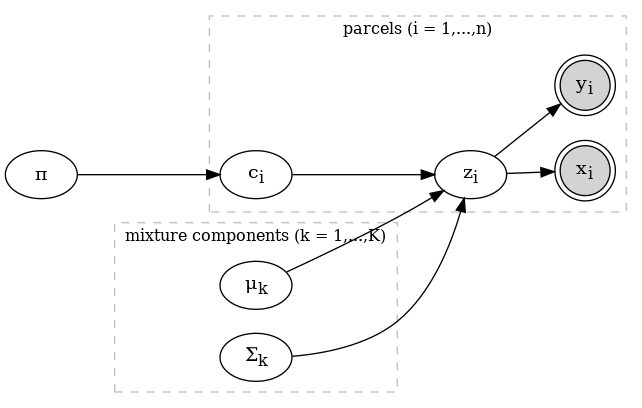
\includegraphics[width=0.7\textwidth]{../images/miwae_graphical_model.png}
          \caption{SemiSupMIWAE Structure.}
        \end{figure}
        \vspace{0.2cm}
        \begin{figure}
            \centering
            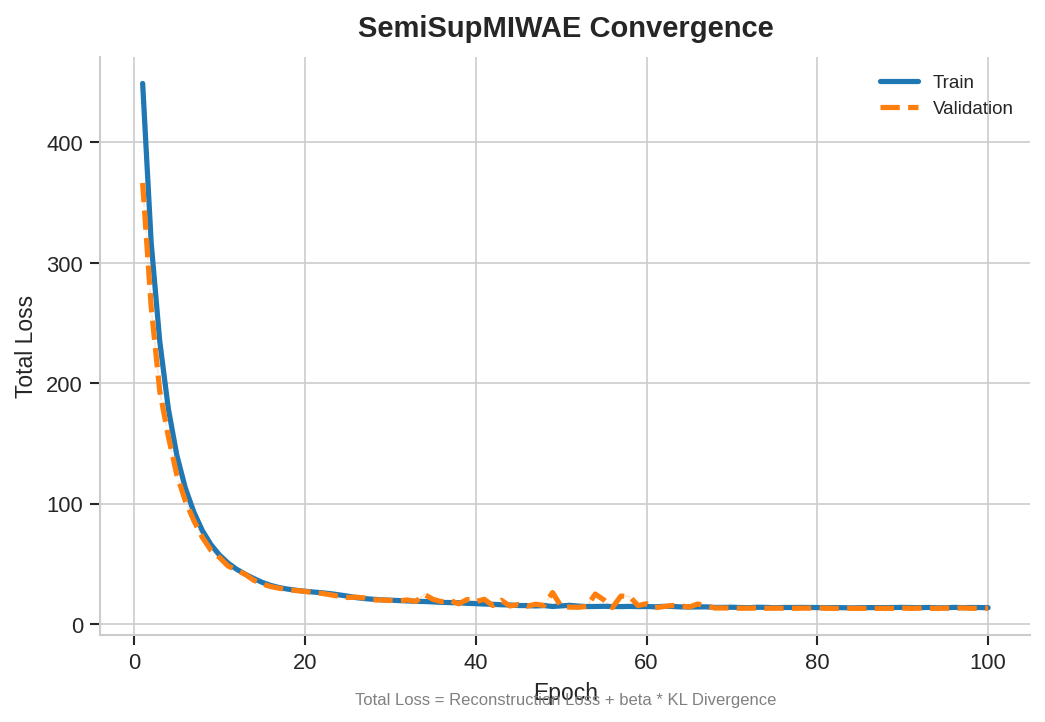
\includegraphics[width=0.7\textwidth]{../images/convergence_loss.png}
            \caption{Convergence (Neg. ELBO) over 50 epochs.}
        \end{figure}
      \end{block}
      \vfill
      \end{minipage}
    \end{column}
    
    % Spacer
    \begin{column}{0.02\paperwidth}\end{column}

    % --- COLUMN 2 ---
    \begin{column}{0.31\paperwidth}
      \begin{minipage}[t][0.79\paperheight][s]{\linewidth}
      \begin{block}{Predictive Performance}
        Evaluated on a 20\% held-out set.
        \vspace{0.5cm}
        \begin{table}
          \centering
          \begin{tabular}{lr}
            \toprule
            \textbf{Metric} & \textbf{Value} \\
            \midrule
            Avg. Log Posterior $p(y \mid x)$ & $-2.28$ \\
            RMSE & \$24.6 Million \\
            MAE & \$2.18 Million \\
            Median Absolute Error & \$128,000 \\
            95th Percentile Error & \$60 Million \\
            \bottomrule
          \end{tabular}
          \caption{Predictive metrics.}
        \end{table}
      \end{block}
      \vfill

      \begin{block}{Residual Analysis}
        \begin{figure}
          \centering
          \begin{tabular}{cc}
             \raisebox{-0.5\height}{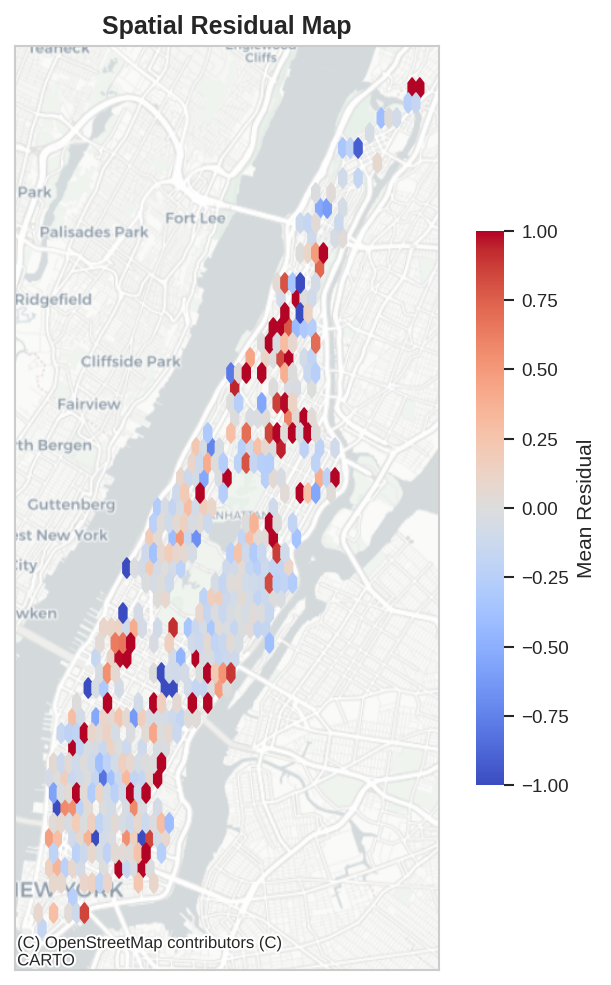
\includegraphics[width=0.45\textwidth]{../images/residuals_spatial_map.png}} & 
             \raisebox{-0.5\height}{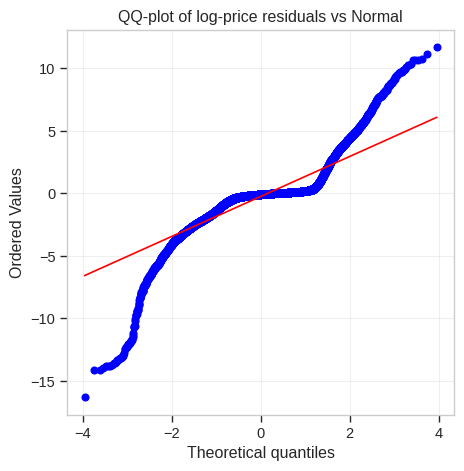
\includegraphics[width=0.45\textwidth]{../images/miwae_residuals_qq.png}} \\
             \small Spatial Bias & \small QQ Plot \\
             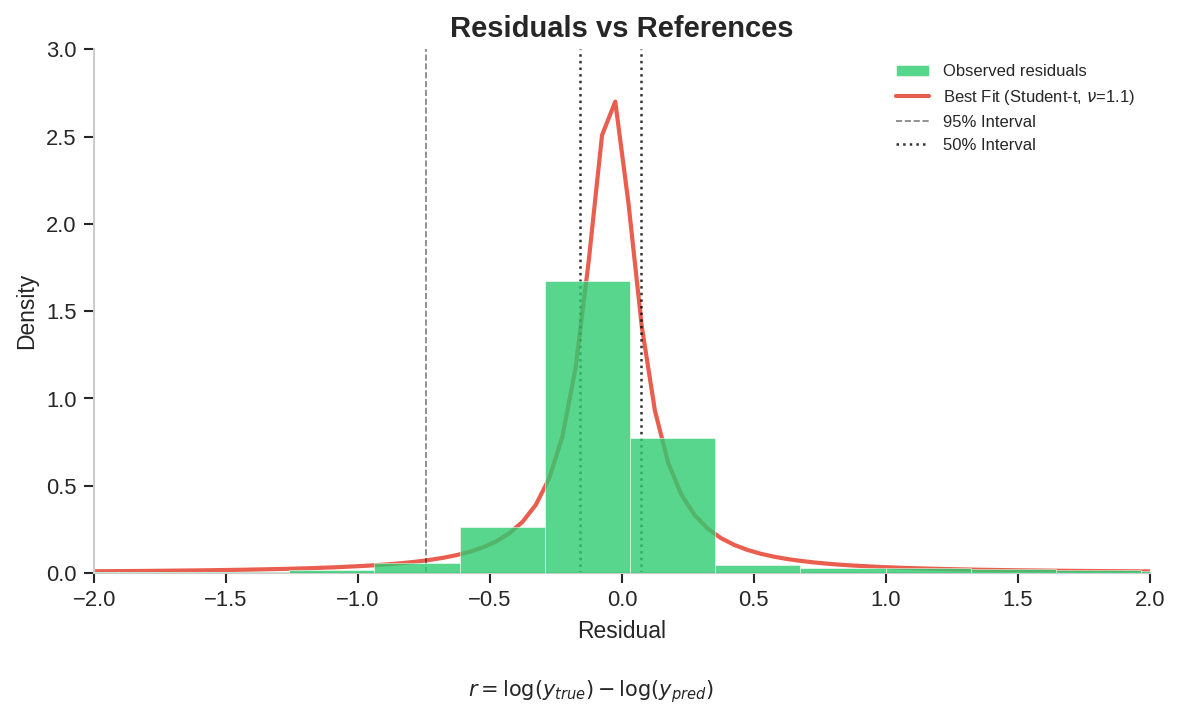
\includegraphics[width=0.45\textwidth]{../images/residuals_hist_references.png} & 
             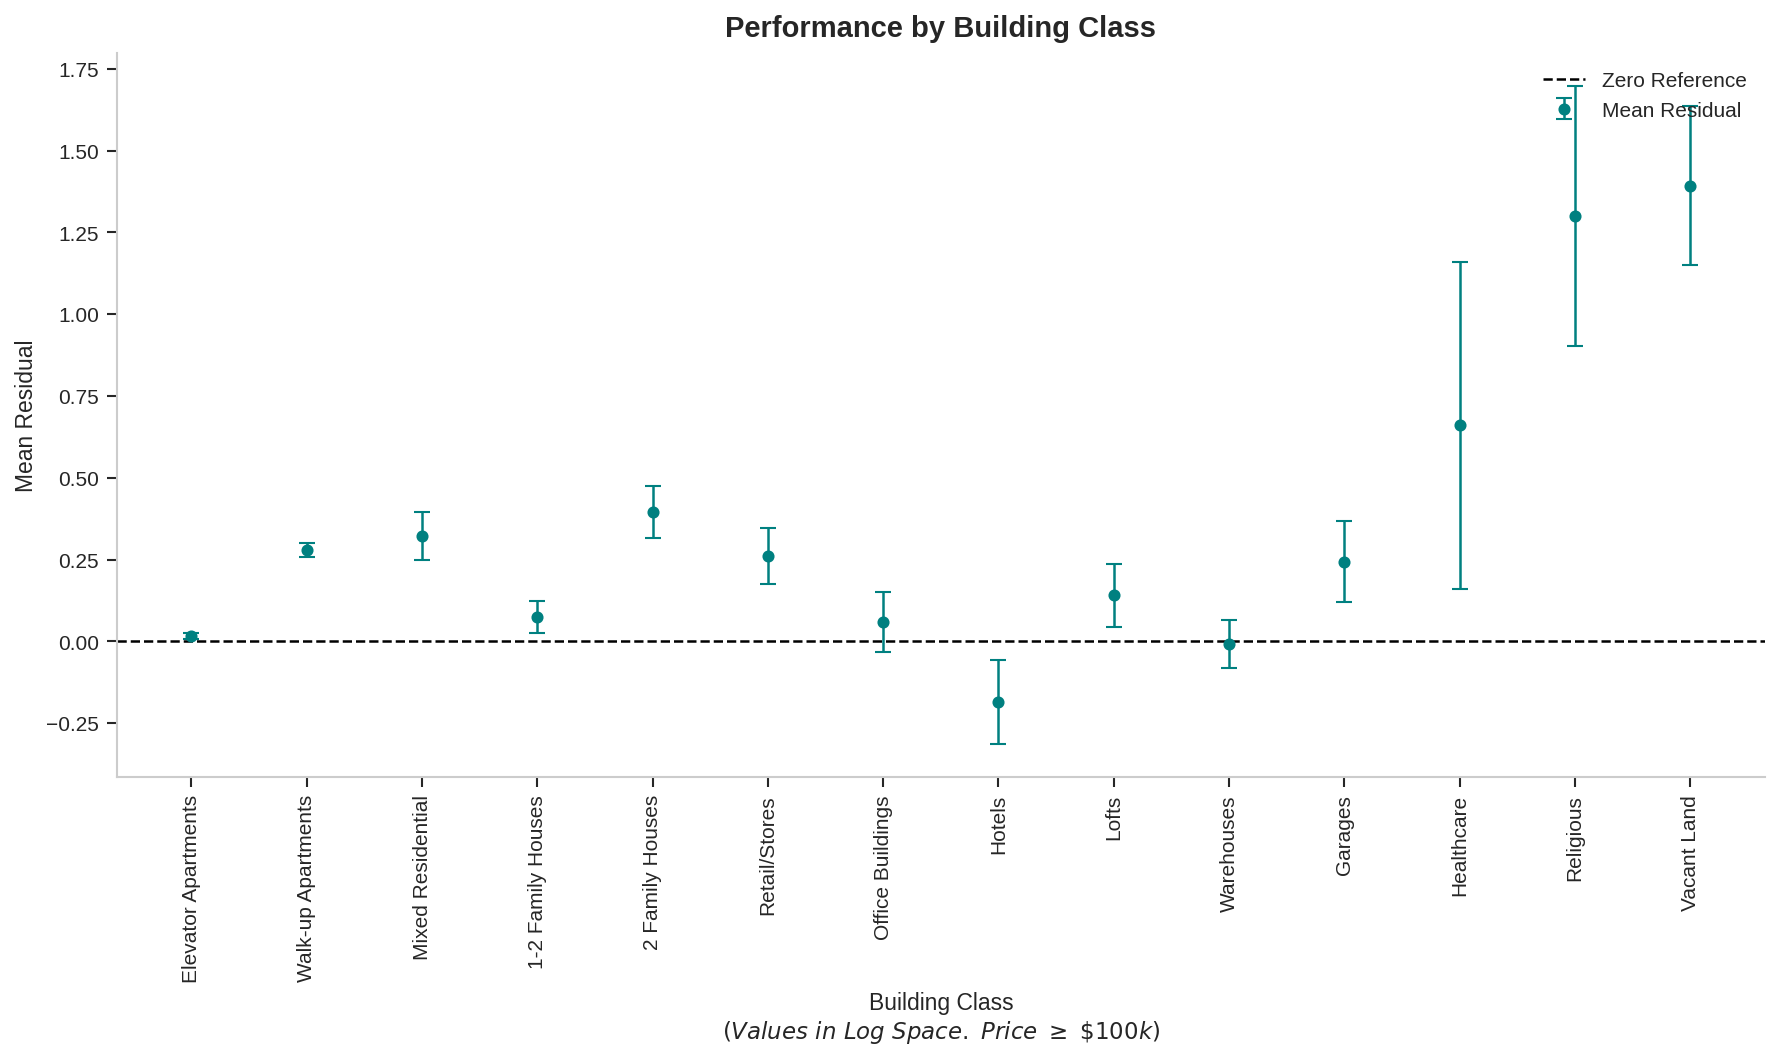
\includegraphics[width=0.45\textwidth]{../images/residuals_by_bldg_class.png} \\
             \tiny Kurtosis = 9.27 (Heavy Tails) & \small Residuals by Building Class
          \end{tabular}
          \caption{Diagnostics: Spatial clustering (left) and QQ Plot (right).}
        \end{figure}
        \vspace{1.5cm}
        \begin{figure}
          \centering
          \begin{tabular}{cc}
             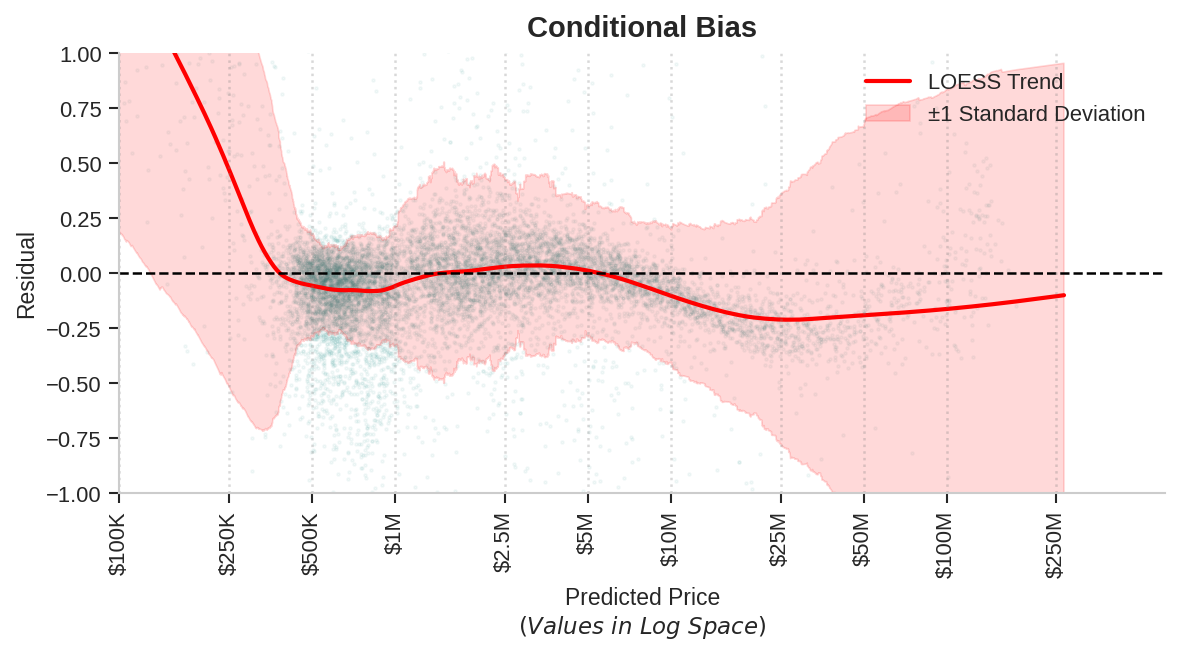
\includegraphics[width=0.45\textwidth]{../images/residuals_vs_pred_bias.png} & 
             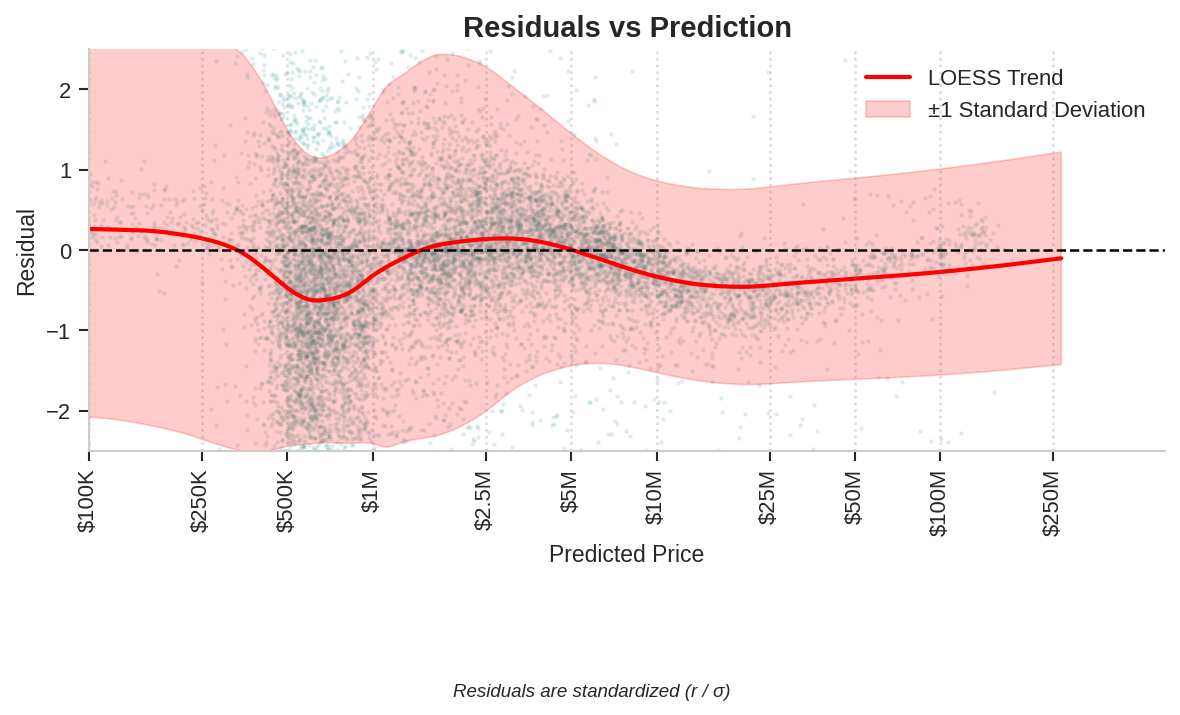
\includegraphics[width=0.45\textwidth]{../images/residuals_standardized_vs_pred.png} \\
             \small Bias vs. Prediction & \small Heteroscedasticity
          \end{tabular}
          \caption{Model Assumption Checks: Conditional Bias (left) and Homoscedasticity (right).}
        \end{figure}
      \end{block}
      \vfill
      \end{minipage}
    \end{column}

    % Spacer
    \begin{column}{0.02\paperwidth}\end{column}

    % --- COLUMN 3 ---
    \begin{column}{0.31\paperwidth}
      \begin{minipage}[t][0.79\paperheight][s]{\linewidth}
      \begin{block}{Latent Space Analysis}
        \textbf{Primary Dimension (49.9\% var)}: Encodes market trends and volume. \\
        \textbf{Secondary Dimension (30.2\% var)}: Separates building classes.
        
        \vfill
        \begin{figure}
          \centering
          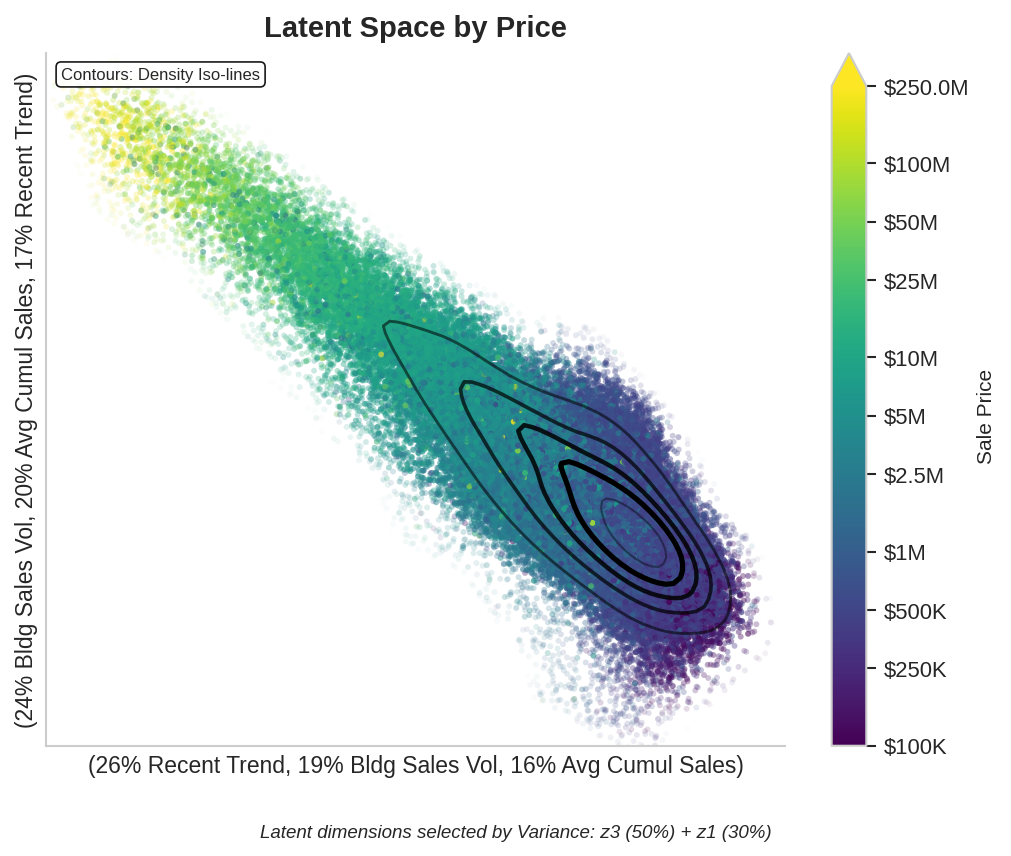
\includegraphics[width=0.8\textwidth]{../images/latent_space_price.png}
          \caption{Latents by Price Decile: Smooth gradient tracks value.}
        \end{figure}

        \vfill
        \begin{figure}
          \centering
          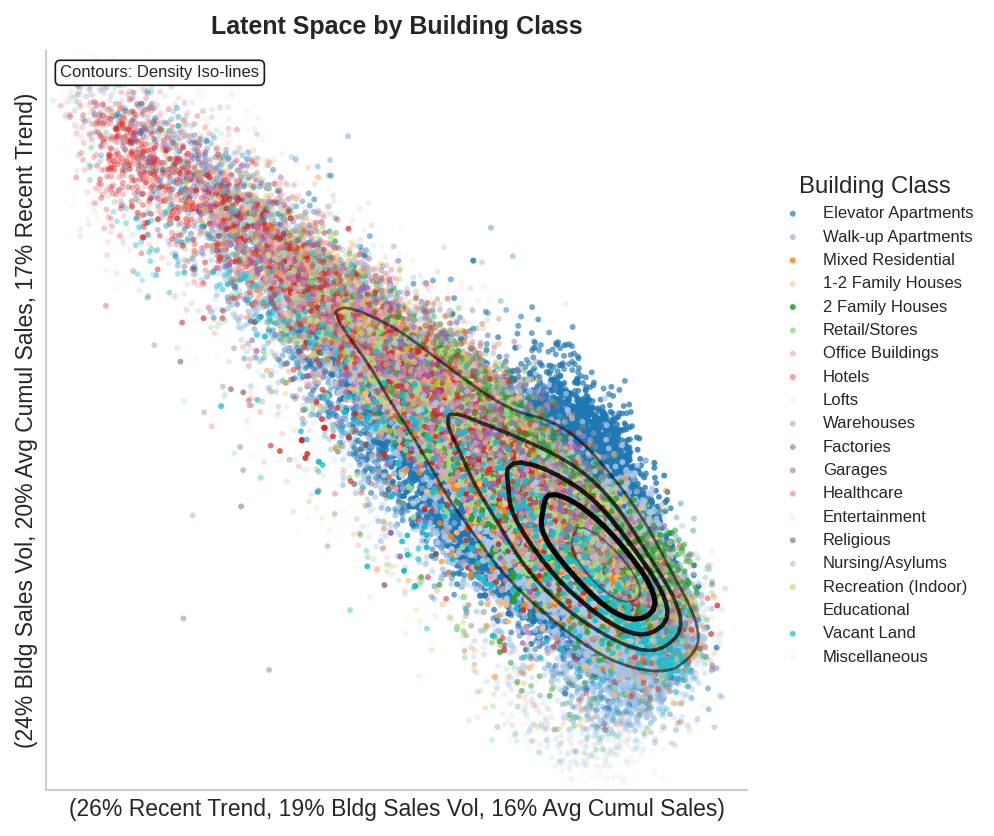
\includegraphics[width=0.8\textwidth]{../images/latent_space_bldg.png}
          \caption{Latents by Building Class: Identifiable striations.}
        \end{figure}
      \end{block}

%       \begin{block}{Discussion \& Future Work}
%         \begin{itemize}
%           \item \textbf{Findings}: Latents organize properties by value type, but Gaussian head misses tails (residual analysis). % TODO: VERIFY R^2 (Prev: 0.27)
%             \begin{center}
%               
\includegraphics[width=0.6\textwidth]{../images/residuals_qq_simple.png}
%             \end{center}
%           \item \textbf{Future Work}:
%             \begin{itemize}
%               \item \textbf{Heavier Tails}: Replace Gaussian likelihood with Student-t.
%               \item \textbf{Spatial}: Add Graph Neural Networks for neighborhood effects.
%               \item \textbf{Visuals}: Overlay Gaussian on residual plots for kurtosis reference.
%             \end{itemize}
%         \end{itemize}
%       \end{block}
     \end{minipage}
     \end{column}
  \end{columns}
\end{frame}
\end{document}
